\subsection{Backend megvalósítása}

\subsubsection{Adathozzáférési réteg - DAL}

\paragraph{Eloquent ORM:}
A backenden, a Laravel keretrendszerben az adathozzáférési réteget az Eloquent nevezetű ORM (Object Relational Mapper) biztosítja. Az Eloquent segítségével a PHP objektumokat és az adatbázis táblákat lehet egymáshoz kapcsolni. Az Eloquent ORM segítségével lehetőség van migrációk írására, modellek, seeder-ek, factory-k, stb. létrehozására.

\paragraph{Migrációk:}
A migrációs fájlok segítségével a táblák struktúráját lehet definiálni. Ez különösen hasznos a hordozhatóság szempontjából, mivel a migrációk segítségével a fejlesztők könnyen telepíthetik az alkalmazást a különböző adatbáziskezelőket használó környezetekbe. Mi a backend fejlesztése során a MySQL adatbázist használtunk.

Külön kiemelendő, hogy a Laravelben lehetőség nyílik UUID-k haználatára integer ID-k helyett amit ki is használtunk. Ennek előnye, hogy ez egy 36 hosszú alkalmazás szinten egyedi szöveges azonosítót generál minden rekordhoz, így kevésbé kikövetkezethető az adatbázis tartalma, mely nagyobb biztonságot nyújt. A globális egyediség az ütközések elkerülése végett is előnyös. 

\paragraph{Modellek:}
A modellek az táblákat reprezentálják az alkalmazásban objektum orientált módon, ahol maga az osztály a tábla, az osztály példányok pedig a tábla sorai. A modellek segítségével lehetőség van az adatok lekérdezésére, frissítésére, törlésére, valamint az adatok közötti kapcsolatok definiálására, így az 1:1 kapcsolatok, 1:N kapcsolatok, N:M kapcsolatok is könnyen definiálhatóak.

Ezen kívűl a Like és Comment modelleknél a beépített Morph relációkat is használtuk, melyek segítségével egy táblához több másik tábla is kapcsolódhat (polymorphic relationship). Ehhez a Laravel minden táblához egy \textit{\_type} és egy \textit{\_id} mezőt ad hozzá (pl: \texttt{likeable\_type} és \texttt{likeable\_id}), melyek segítségével azonosítani lehet a kapcsolódó táblát és azon belül az egyedi azonosítót.

Az alkalmazásunkban található modellek áttekintő ábrája a \ref{fig:models}. ábrán látható.

\begin{figure}[H]
    \centering
    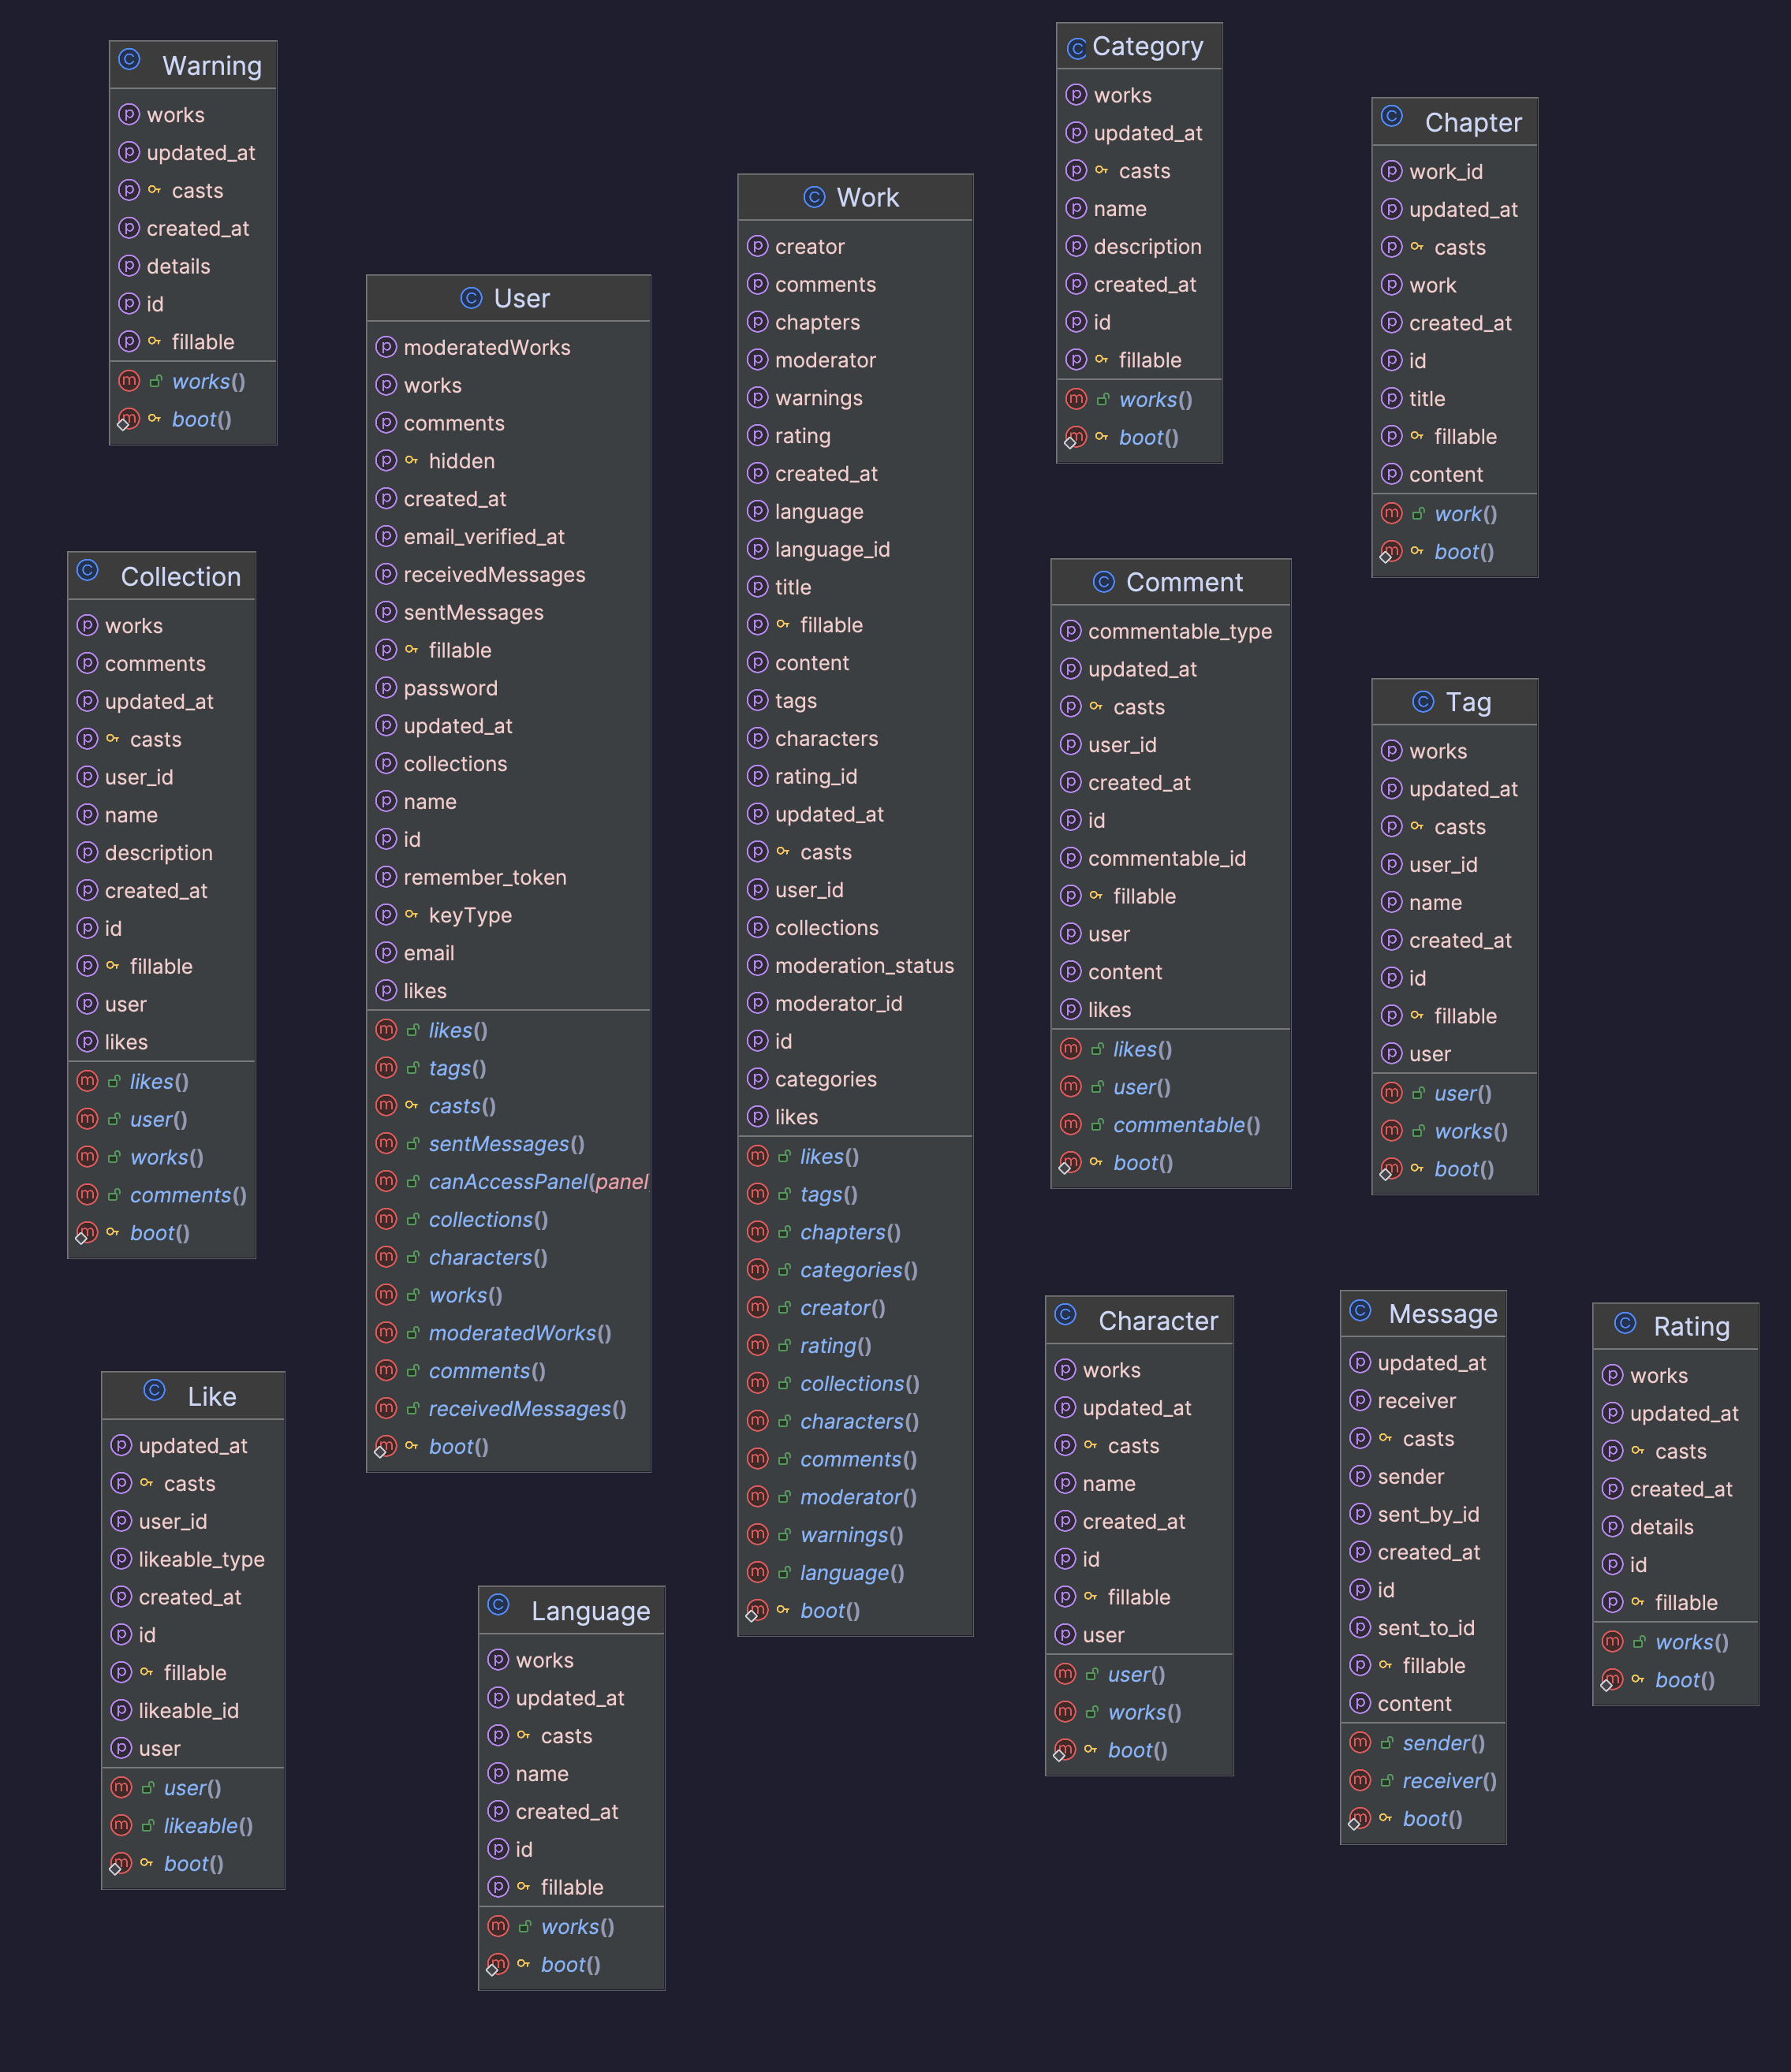
\includegraphics[scale=0.1]{./figures/models.png}
    \caption{Az alkalmazás modelljei}
    \label{fig:models}
\end{figure}


\paragraph{Factory-k:}
A factory-k segítségével lehetőség van tesztadatok generálására az adatbázisba. A factory-k segítségével lehetőség van a modellekhez kapcsolódó adatok generálására, amelyeket a tesztelés során lehet használni. Ehhez a Laravel a Faker nevű könyvtárat használja, amely segítségével különböző típusú hamis, de struktúrális tekintetben helytálló adatokat lehet generálni.

\paragraph{Seeder-ek:} A factory osztályok segítségével generált adatokat a seeder-ek segítségével lehet az adatbázisba betölteni, meghatározott mennyiségben és kapcsolatokkal. Külön jelentősége volt a \texttt{PermissionSeeder}-nek mely az alkalmazás jogosultságait definiálja.

\subsubsection{Üzleti logika réteg - BLL}

Az üzleti logikai réteg a Laravel keretrendszerben a vezérlőkön (Controller) és a hozzájuk kapcsolódó komponenseken keresztül valósul meg. Ez a réteg felel az alkalmazás alapvető működési logikájáért, amely az adatbázis-interakciók és a felhasználói kérések között helyezkedik el.
\paragraph{Vezérlők (Controllers)}

A vezérlők a Laravel MVC (Model-View-Controller) architektúrájának központi elemei, amelyek a beérkező \texttt{HTTP}-kéréseket kezelik és a megfelelő válaszokat generálják.
A projektben mindegyik modellre készítettünk egy \texttt{<modell neve>Controller} névkonvenciójú vezérlő osztályt. A vezérlők a Laravel keretrendszerben a \texttt{app/Http/Controllers} könyvtárban találhatók. Minden vezérlő osztály a Laravel saját Controller bázisosztályból származik, amely alapvető funkciókat biztosít. A vezérlők metódusai a különböző CRUD \texttt{HTTP}-kérésekhez (\texttt{GET, POST, PUT, DELETE}) kapcsolódnak, és az útvonalak (routes) segítségével érhetők el.


\paragraph{Útvonalak és REST API (Routing and REST API)}

Az útvonalak határozzák meg, hogy a beérkező \texttt{HTTP}-kérések mely vezérlők mely metódusait hívják meg. A Laravelben az útvonalak a routes könyvtárban találhatók, és különböző fájlokban definiálhatók. Az alkalmazásunk útvonalai az api.php fájlban találhatóak, és alább látható belőle egy kódrészlet.
\begin{lstlisting}[language=php][]
    // api.php
    Route::group(['middleware' => 'auth:sanctum'], function () {
    Route::get('/user', function (Request $request) {
        return $request->user();
    });
        Route::post('/works', [WorkController::class, 'store'])
                            ->can('create', Work::class);
        Route::put('/works/{work}', [WorkController::class, 'update'])
                            ->can('update', 'work');
        Route::delete('/works/{work}', [WorkController::class, 'destroy'])
                            ->can('delete', 'work');
    });
    Route::get('/works', [WorkController::class, 'index'])
                            ->can('view', Work::class);
    Route::get('/works/{work}', [WorkController::class, 'show'])
                            ->can('view', Work::class);
\end{lstlisting}

E példában az útvonalak a WorkController különböző metódusaira irányítják a kéréseket, és az \textbf{auth:sanctum} middleware biztosítja, hogy csak hitelesített felhasználók férhessenek hozzá ezekhez az útvonalakhoz.

A REST API (Representational State Transfer Application Programming Interface) egy architektúrális stílus, amely lehetővé teszi az erőforrások \texttt{HTTP} protokollon keresztüli elérését és manipulálását. A Laravelben az útvonalak és vezérlők segítségével valósítható meg a REST API-k kialakítása.


\paragraph{Kérések (Requests)}
A Laravel Request osztálya biztosítja, hogy objektumorientált módon lehessen kezelni, az alkalmazás által aktuálisan kezelt \texttt{HTTP}-kérelmeket, valamint a kéréssel együtt elküldött cookie-k és fájlok lekérdezését. A \texttt{HTTP} kérések példányainak kiosztását DI (Dependency Injection) segítségével oldja meg a Laravel.

\paragraph{Válaszok (Responses)}
A Response példányok használata, lehetővé teszi a válasz \texttt{HTTP} státuszkódjának és fejlécének testreszabását. Minden modellhez tartozó Response példány a Laravel saját Response osztályából örököl, amely számos módszert biztosít a \texttt{HTTP}-válaszok testreszabására, mint egyfajt DTO (Data Transfer Object) használata.


\paragraph{Autómatikus értesítés moderáció eredményéről:}
A Laravel egyszerű módot biztosít az e-mailek küldésére mindenféle gond és nehézség nélkül a Mailable osztály használatával.
A Laravel Mail API a népszerű Swiftmailer könyvtárra épült. Mi úgy konfiguráltuk, hogy SMTP-t használjon, de sok egyéb konfigurációval is lehet használni (Pl.: Mailgun, Amazon SES).
A Mail konfigurációkat a backend projekt gyökérkönyvtárában megtalálható \texttt{.env} fájlban kell beállítani az alábbi módon:


\begin{lstlisting}[language=php]
    MAIL_MAILER=smtp
    MAIL_HOST=mailpit
    MAIL_PORT=1025
    MAIL_USERNAME=null
    MAIL_PASSWORD=null
    MAIL_ENCRYPTION=null
    MAIL_FROM_ADDRESS="hello@example.com"
    MAIL_FROM_NAME="${APP_NAME}"
\end{lstlisting}
Az alábbi parancs kiadásával tudjuk létrehozni a saját Mailable osztályunk és a hozzá tartozó email-levél sablon fájlunkat.
\begin{center}
   \begin{verbatim}
    $ php artisan make:mail ModerationMail  --markdown=emails.moderations
    \end{verbatim}
\end{center}

A ModerationMailable osztályból biztosítom a sablon számára a paramétereket, melyeknek értékeit megszeretnénk jeleníteni az email-ben. Ilyen paraméterek jelenleg a \textbf{work}, ami az adott munka objektumát reprezentálja, és a címét és az azonosítóját kérdezem le a sablonban. Valamint a \textbf{creator}, ami pedig az a User példány, amelyik létrehozta a munkát.

Miután elkészült a saját Mailable osztályunk és a hozzátartozó markdown sablont is megformáztuk, akkor már csak a kiküldés implementálása hiányzik. Erre használható a Laravel Mail Facade. Rengeteg metódussal rendelkezik, de a legfontosabb a \textbf{to} metódus. Ez a metódus határozza meg, hogy az email hova kerül elküldésre. Átadhatjuk a felhasználó email címét paraméterként, és a Laravel elküldi az emailt a megadott email címre. 

A következő fontos metódus a \textbf{send} metódus. Ez a metódus lehetővé teszi számunkra, hogy megadjunk egy Mailable üzenet példányt, tehát itt adtuk meg a korábban létrehozott Mailable osztályt.
A levél elküldését a Work modell osztályának updating metódusában implementáltuk, mivel moderálást csakis munkákra lehet kérni, és amikor a ModerationStatus enumjának értéke \texttt{APPROVED} vagy \texttt{EDIT\_REQUESTED} értékek valamelyikét veszi fel, akkor kell kiküldenünk az emailt.

A Laravel megkönnyíti az emailek tesztelését azáltal, hogy third-party könyvtárakat szolgáltat, mint például a Laravel mailpit, vagy a Mailtrap. Ezek a szolgáltatások egy hamis SMTP szervert biztosítanak, ahonnan tesztelhetjük és ellenőrizhetjük, hogy az emailek helyesen vannak\-e formázva. Értelemszerűen meg kell változtatni a mail konfigurációkat az .env fájlban, hogy valamely hamis SMTP szerver hitelesítő adatait használja. A Mailtrap használatával például vizuálisan láthatjuk, hogyan van formázva az email és emiatt döntöttünk mi is e mellett.


\paragraph{Authentikáció:} Az authentikációra a Laravel Breeze \cite{LaravelBreeze} csomagot használtuk, mely egy minimális authentikációs rendszert biztosít. Az authentikációhoz szükséges routokat, controllereket, view-kat és middleware-eket a csomag automatikusan generálja. Az authentikációhoz szükséges adatbázis táblákat is a csomag generálja, így a felhasználók regisztrációja, bejelentkezése, jelszó visszaállítása, stb. egyszerűen megvalósítható.

A Breeze alapvetően Session alapú CSRF és CORS védelemmel rendelkező authentikációt biztosít a frontendek számára. Azonban maga a Breeze egy másik csomagra a Laravel Sanctum-ra \cite{LaravelSanctum} épít. Ennek előnye, hogy a Sanctum biztosít API Token alapú authentikációt is melyet a mobil kliens így ki tudott használni.\\

\paragraph{Authorizáció:} Az authorizációra a Spatie cég által fejlesztett és karbantartott Laravel Permission csomagot \cite{LaravelPermissions} használtuk. A csomag segítségével lehetőség van jogosultságok (permissions) definiálására, azokhoz szerepkörök (roles) rendelésére, valamint a jogosultságok és szerepkörök alapján az authorizáció megvalósítására. A csomag a Laravel Policy-ket használja az authorizáció megvalósítására, amelyek segítségével a jogosultságokat és szerepköröket a modellekhez lehet rendelni.

Ennek előnye hogy ellenőrzéskor csak a jogosultság meglétét kell ellenőrizni, azonban a jogosultságok egységesen kioszthatók role-ok segítségével. Az alkalmazás 3 szerepkört valósít meg, melyek a \texttt{Registered}, \texttt{Moderator} és \texttt{Admin}. Az admin az alkalmazás ServiceProvider-ében minden ellenőrzésen automatikusan átengedésre kerül, így nem kell az össze jogosultságot hozzárendelni.\\


\subsubsection{Tesztelés}

\paragraph{Laravel Pest}

A Laravel Pest egy modern PHP tesztelési keretrendszer, amely a Laravel alkalmazások tesztelését egyszerűbbé és olvashatóbbá teszi. A Pest a PHPUnit alapjaira épül, de letisztultabb szintaxist és fejlett funkciókat kínál, amelyek megkönnyítik a tesztek írását és karbantartását.

\paragraph{A Pest jellemzői}

\begin{itemize} \item \textbf{Egyszerű szintaxis:} A Pest minimalista megközelítése révén a tesztek könnyen olvashatók és írhatók, csökkentve a boilerplate kód mennyiségét. \item \textbf{Gyors telepítés:} A Pest gyorsan integrálható meglévő Laravel projektekbe, lehetővé téve a zökkenőmentes átállást vagy párhuzamos használatot a PHPUnit-nal. \item \textbf{Fejlett funkciók:} Beépített támogatás a párhuzamos teszteléshez, mutációs teszteléshez és architektúra teszteléshez, amelyek növelik a tesztelés hatékonyságát és megbízhatóságát. \end{itemize}

A Pest használata a Laravel alkalmazások tesztelésére modern és hatékony megközelítést kínál, amely növeli a fejlesztés minőségét és sebességét.

Ezért választottuk a backend oldalon is a Pest\-et az autentikáció és a vezérlők (controller), valamint a Request-s unit tesztelésére.

\subsubsection{Admin felület}

Bár nem külön alkalmazás réteg de megemlítendő, hogy az admin felület megvalósítására a FilamentPHP csomagot \cite{FilamentPHP} használtuk a backend oldalon. Előnye, hogy a modell osztályokhoz definiálhatóak úgynevezett filament resource-ok melyek az admin felületen megjelenő mezőket és azok viselkedését definiálják. A csomag segítségével lehetőség van a modellek szerkesztésére, törlésére, listázására, stb. Az admin felület a \ref{fig:admin}. ábrán látható.

\begin{figure}[H]
    \centering
    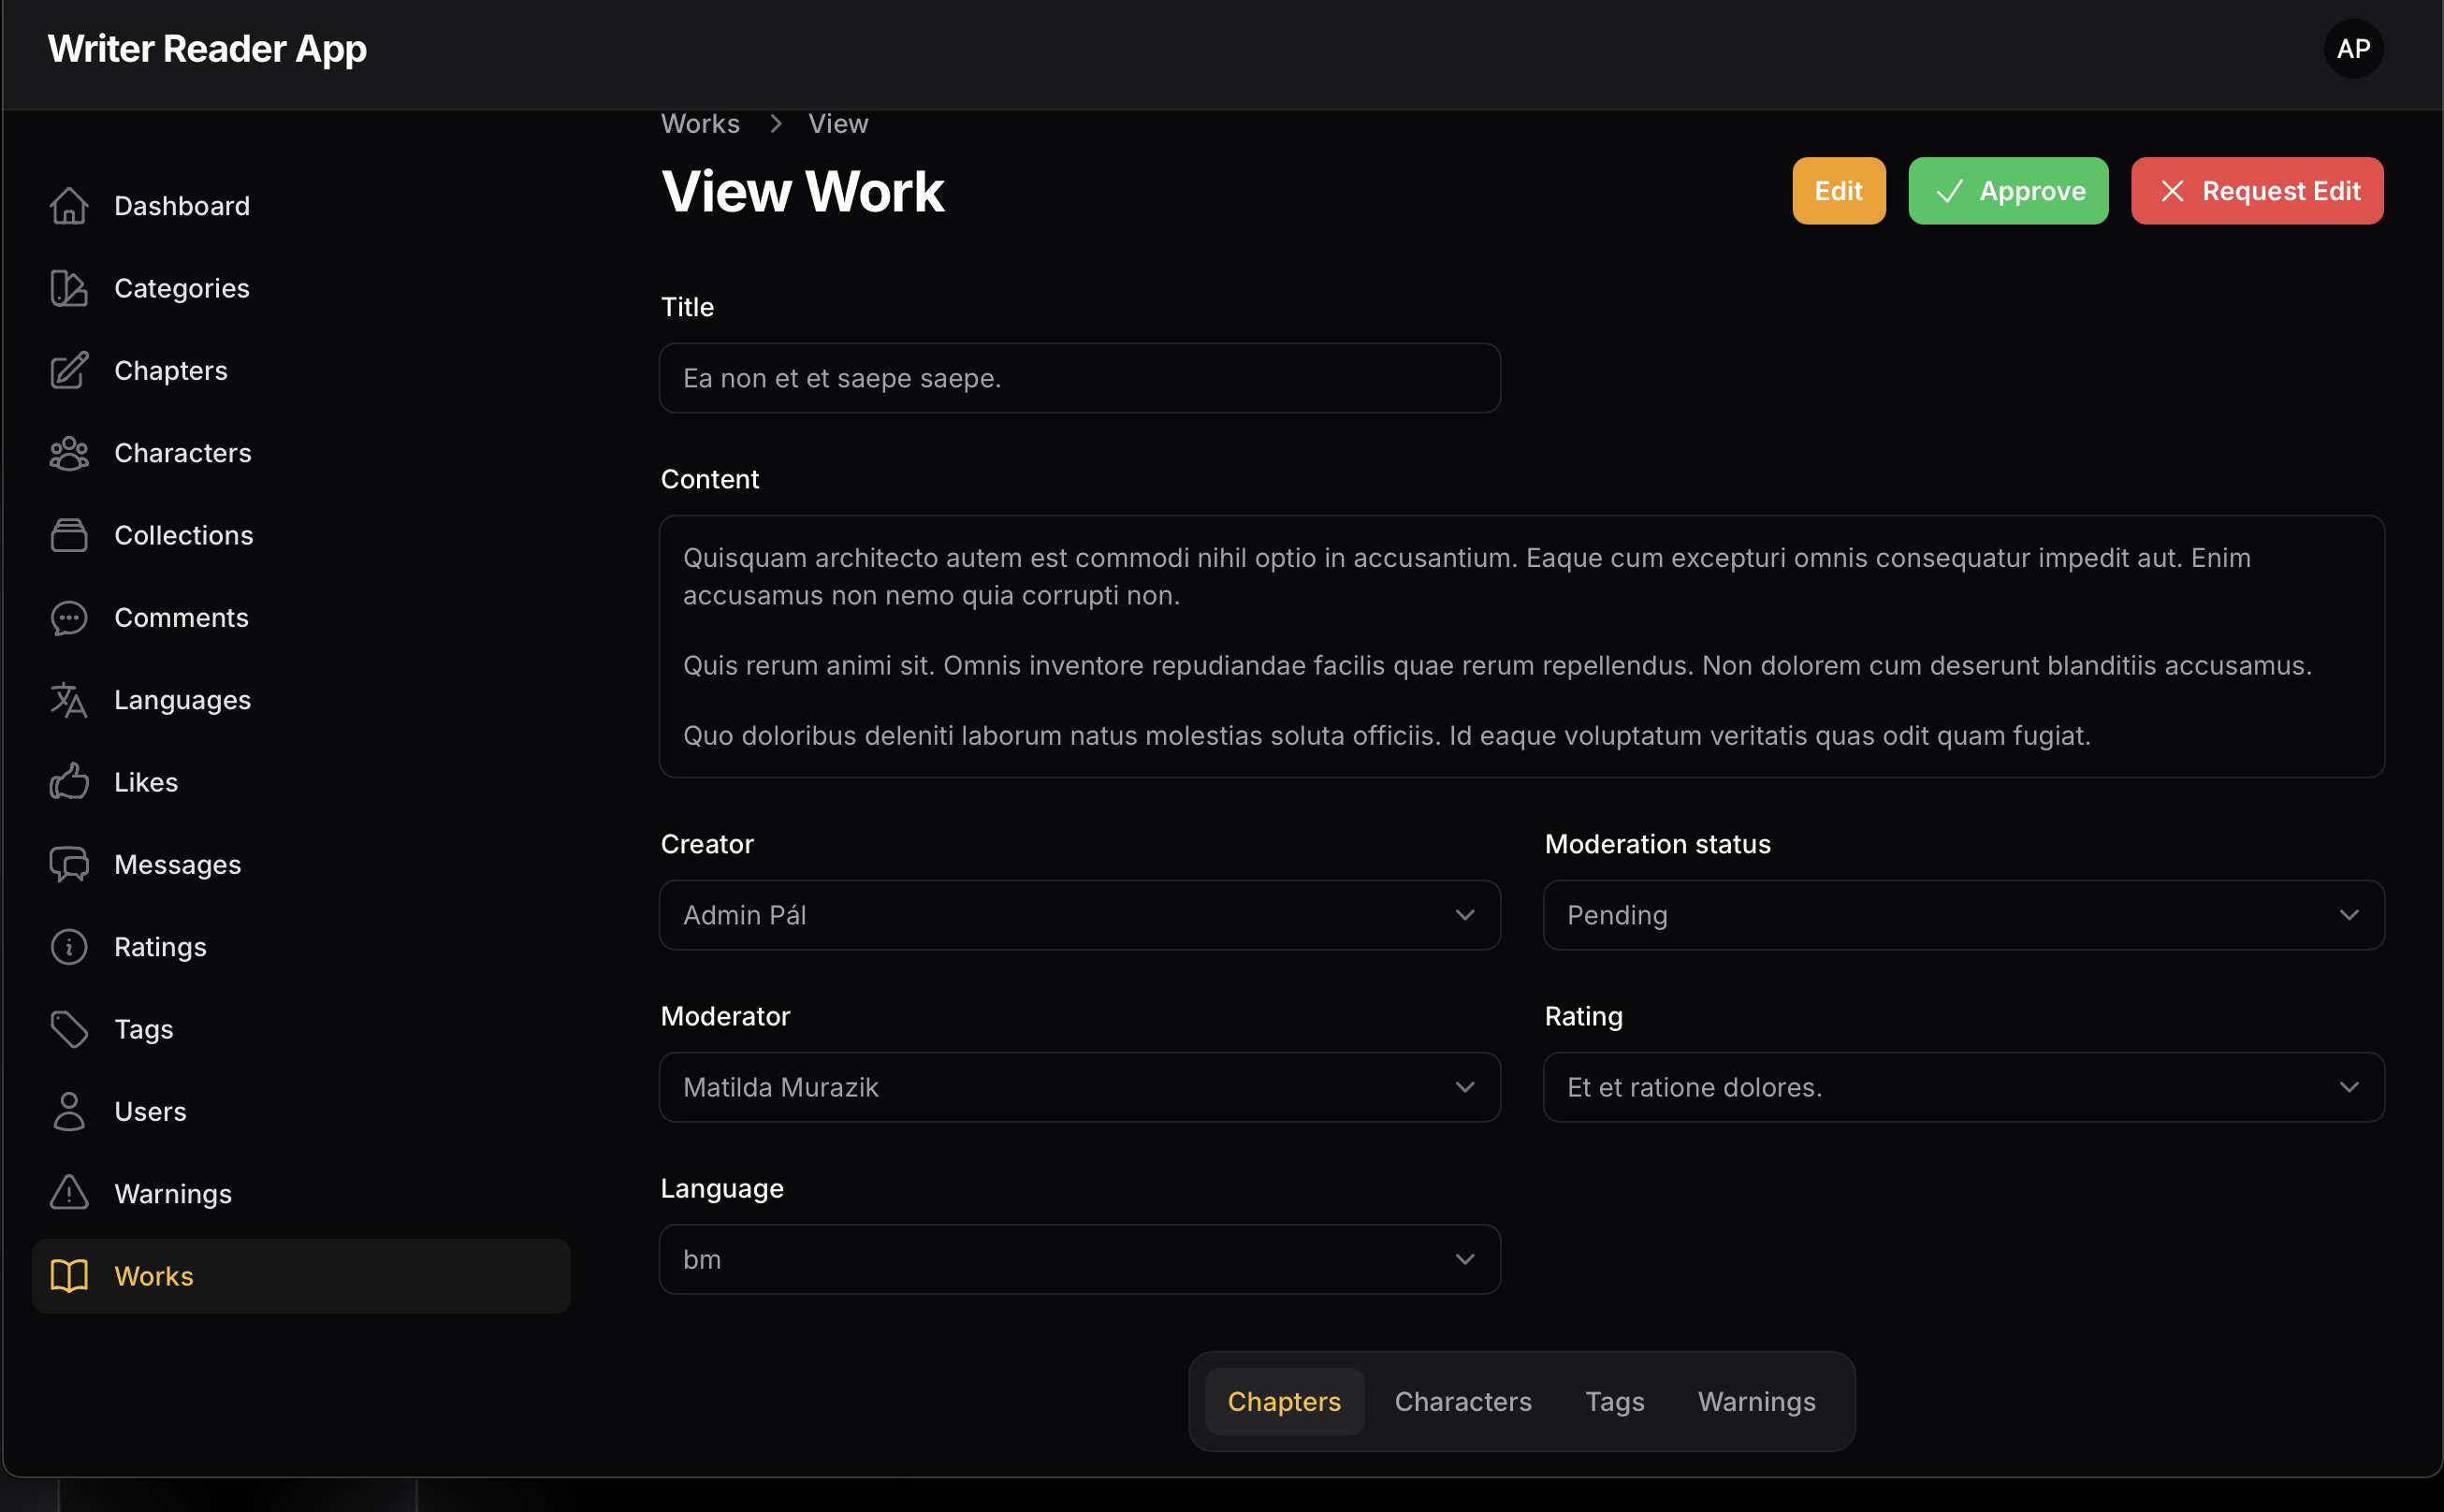
\includegraphics[scale=0.25]{./figures/admin-panel.png}
    \caption{FilamentPHP admin felület}
    \label{fig:admin}
\end{figure}

Az admin felülethez csak moderátor és admin jogosultságú felhasználó férhet hozzá. Azon belül az egyes modellek-hez való hozzáférést a policy osztályok szabályozzák de felülírható külön a filament resource-okon keresztül is.

Ezen kívűl az adminfelületen került megvalósításra a művek jóváhagyása is melyekre a moderátoroknak van jogosultságuk. A jóváhagyás után a művek publikussá válnak és megjelennek a felhasználók számára is, valamint automatikusan email értesítés küldődik a mű létrehozójának.
